\documentclass{article}
\usepackage[utf8]{inputenc}
\usepackage{graphicx}
\usepackage[simplified]{pgf-umlcd}
\usepackage{tikz}
\usepackage{multirow}
\usepackage{float}
\usetikzlibrary{positioning,fit,calc,arrows.meta, shapes}
\usepackage{wrapfig}
\usepackage{listings}
\usepackage{hyperref}
\usepackage{amsmath}
\graphicspath{ {images/} }
\usepackage{array}
\newcolumntype{L}[1]{>{\raggedright\let\newline\\\arraybackslash\hspace{0pt}}m{#1}}
\newcolumntype{C}[1]{>{\centering\let\newline\\\arraybackslash\hspace{0pt}}m{#1}}
\newcolumntype{R}[1]{>{\raggedleft\let\newline\\\arraybackslash\hspace{0pt}}m{#1}}

%Tot això hauria d'anar en un pkg, però no sé com és fa
\newcommand*{\assignatura}[1]{\gdef\1assignatura{#1}}
\newcommand*{\grup}[1]{\gdef\3grup{#1}}
\newcommand*{\professorat}[1]{\gdef\4professorat{#1}}
\renewcommand{\tablename}{Taula}
\renewcommand{\title}[1]{\gdef\5title{#1}}
\renewcommand{\author}[1]{\gdef\6author{#1}}
\renewcommand{\date}[1]{\gdef\7date{#1}}
\renewcommand{\contentsname}{Índex}
\renewcommand{\listfigurename}{Llista d'imatges}
\renewcommand{\listtablename}{Llista de Taules}
\renewcommand{\maketitle}{ %fa el maketitle de nou
    \begin{titlepage}
        \raggedright{UNIVERSITAT DE LLEIDA \\
            Escola Politècnica Superior \\
            Grau en Enginyeria Informàtica\\
            \1assignatura\\}
            \vspace{5cm}
            \centering\huge{\5title \\}
            \vspace{3cm}
            \large{\6author} \\
            \normalsize{\3grup}
            \vfill
            Professorat : \4professorat \\
            Data : \7date
\end{titlepage}}
%Emplenar a partir d'aquí per a fer el títol : no se com es fa el package
%S'han de renombrar totes, inclús date, si un camp es deixa en blanc no apareix
\renewcommand{\figurename}{Figura}
\title{Anàlisi de la xarxa mitjançant l'analitzador de protocols de xarxa Wireshark}
\author{Sergi Simón Balcells\\21040111X}
\date{Diumenge 19 de Maig}
\assignatura{XARXES}
\professorat{E. Guitart, C. Mateu}
\grup{GM3}

%Comença el document
\begin{document}
\maketitle
\thispagestyle{empty}

\newpage
\pagenumbering{roman}
\tableofcontents
\listoffigures
\listoftables
\newpage
\pagenumbering{arabic}
\section{Introducció}
\section{Caractarístiques de la xarxa}
% Anàlisi paquest agafar característiques
\subsection{Tipus d'adreçament a la capa de xarxa}
Per a trobar el tipus d'adreçament a la xarxa, s'ha mirat els paquets
tipus ARP per a observar diferents direccions IP de la xarxa.\\
\\
Observant les diferents direccions que es mouen dins de la xarxa, podem
extreure que les direccions de la xarxa són 172.16.x.x, sent les x valors
entre 0 i 255, és a dir, l'adreça de xarxa és 172.16.0.0/16 i per tant
és de  \textbf{classe B}.
\subsection{Adreça de xarxa}
Com s'ha extret en l'anterior secció, la adreça de xarxa és 172.16.0.0.
\subsection{Adreça de broadcast}
Sabent l'adreça de xarxa, podem concloure que
l'adreça de broadcast és 172.16.255.255, ja que aquesta és l'última adreça
disponible de tota la xarxa, és a dir, la part del host de l'adreça a valor
actiu a tots els bits. Inclús amb aquesta informació, per confirmar que no
hi hagi hagut cap error, s'ha procedit a mirar l'adreça de broadcast en els
paquets tipus:\\
\begin{lstlisting}
	    !arp && eth.dst == ff:ff:ff:ff:ff:ff
\end{lstlisting}
Els paquets d'aquest tipus mostren com a direcció IP 172.16.255.255 per destí,
es pot confirmar la informació extreta en aquest apartat.
\subsection{Porta d'enllaç}
S'ha vist en la xarxa que s'empra el protocol DHCP, pel que, primerament
es busca aquels paquests que siguin DHCP ACK:\\
\begin{lstlisting}
		bootp.option.dhcp == 5
\end{lstlisting}
En aquest protocol i en aquest tipus de paquet, es pot trobar la informàció
referent al router,  dins de Bootstrap Protocol (ACK), en opcions de router.
En aquest camp s'especifíca que l'adreça és 172.16.20.1.
\section{Anàlisi de nivell de enllaç i xarxa}
\subsection{Protocols encapsulats en les trames de nivell 2}
Al llarg de tota la trama, es poden veure 2 protocols de nivell 2 de
xarxa, \textbf{Ethernet II} i \textbf{IEEE 802.3 Ethernet}. En les següents
subseccions s'explicarà el tipus d'encapsulament d'aquests
\subsubsection{Ethernet II}
Aquest tipus de trama s'utilitza en l'àmbit general, i es pot trobar en la majoria
de paquets de la captura. La seva estructura segueix la següent:\\
% Taula amb l'estructura
\subsubsection{IEEE 802.3 Ethernet}
Aquesta classe s'utilitza en els protocols de LLC. La seva estructuar és la
següent:
% Taula amb l'estructura
\subsection{Protocols encapsulats en trames de nivell 2}
Per a trobar els diferents protocols utilitzats, s'utilitza la eina de
\textit{Protocol Hierarchy}, accessible dins del menú d'estadístiques del
Wireshark. En aquest menú, podem veure com és divideix els protocols segons els
nivells, començant pel nivell físic, i seguint amb Ethernet. Dins d'aquest menú
es pot veure els següents tipus de paquets, que són: Logical-Link Control (LLC),
Internetwork Packet eXchange (IPX), Internet Protocol Version 6 (IPv6),
Internet Protocol Version 4 (IPv4), Address Resolution Protocol (ARP), que
s'explicaran a continuació, juntament amb el seu valor de tipus.\\
\begin{itemize}
\item ARP, amb valor 0x0806, s'encarrega de resoldre i mantenir de manera automàtoca
la taula d'equivalències entre les adreces MAC i les adreces IP dels nodes o màquines
que es comuniquen.
\item IPv4, amb valor 0x0800, és el protocol per excelència d'Internet. Serveix
per a la identiciació i connexió de nodes.
\item IPv6, amb valor 0x86dd, neix com a un protocol per a substituir IPv4, i
treure els problemes que sorgeixen amb aquest, com és la falta d'adreces, seguretat i
qualitat de servei. Moltes de les seves funcionalitats s'han portat enrere per al
protocol de IPv4.
\item IPX, amb valor 0x8137, s'utilitza per a transmetre datagrames entre els
diferents serviors i els programes de les estacions de treball.
\item LLC, sense valor donat que està encapsulat amb IEEE 802.3 Ethernet i aquest
no te nombre reservat pel tipus, defineix la forma en què les dades són transferides
sobre el medi físic, proporcionant servei a les capes superiors.
\end{itemize}
\subsection{Equips amb adreçament IPX i IPv4}
Per aquesta secció, s'ha mirat manualment els equips que utilitzen IPX 
la seva adreça MAC, i, utilitzant aquesta valor s'ha mirat si hi havia un 
paquet que amb aquesta MAC que utilitzes IPv4 amb la comanda, substituint
l'adreça MAC per aquelles trobades amb l'anterior cerca:\\
\begin{lstlisting}
	(eth.src == 00:00:74:99:b5:0b || eth.dst == 00:00:74:99:b5:0b) && ip
\end{lstlisting}
En la primera cerca dins dels paquests IPX s'ha trobat aquestes adreces i MAC,
com es mostra en la taula \ref{ipx:mac}
\begin{table}[!h]
\centering
\begin{tabular}{|l|r|}
\hline
Adreces IPX &Adreces MAC\\
\hline
00000000.00007499b50b &00:00:74:99:b5:0b\\
\hline
00000000.000074aee28d &00:00:74:ae:e2:8d\\
\hline
00000000.000074b4dbcd &00:00:74:b4:db:cd\\
\hline
00000000.000074d5923f &00:00:74:d5:92:3f\\
\hline
00000000.000074da5833 &00:00:74:da:58:33\\
\hline
00000000.000074dab870 &00:00:74:da:b8:70\\
\hline
00000000.000074ddfd6c &00:00:74:dd:fd:6c\\
\hline
00000000.000074e03eaf &00:00:74:e0:3e:af\\
\hline
00000000.000074e04ef9 &00:00:74:e0:4e:f9\\
\hline
00000000.000074e08d60 &00:00:74:e0:8d:60\\
\hline
00000009.00080228befa &00:08:02:28:be:fa\\
\hline
\end{tabular}
\caption{Adreces MAC i IPX d'equips que utilitzen IPX}
\label{ipx:mac}
\end{table}
Finalment, buscant totes les MACS abans trobades i eliminant aquelles 
files que no s'han trobat paquets d'IPv4 en la trama tenim la taula \ref{ipx:ipv4}.
% Afegir taula script ipx.py
\begin{table}[!h]
\centering
\begin{tabular}{ |c|c|c| }
\hline
Adreça MAC &Adreça IPX &Adreça IPv4\\
\hline
00000000.000074da5833 &00:00:74:da:58:33 &172.16.40.6\\
\hline
00000000.000074ddfd6c &00:00:74:dd:fd:6c &172.16.40.11\\
\hline
00000000.000074e04ef9 &00:00:74:e0:4e:f9 &172.16.40.4\\
\hline
00000000.000074e08d60 &00:00:74:e0:8d:60 &172.16.40.3\\
\hline
\end{tabular}
\caption{Taula de adreces IPX que han utilitat protocol IPv4 i ha sigut captat.}
\label{ipx:ipv4}
\end{table}
\subsection{Adreces IPv4 dels nodes que envien paquests IPv6 a ff02::1}
En aquesta subsecció s'explicarà com s'ha trobat aquells equips que envien
paquets d'IPv6 a tots els nodes de l'enllaç local, es a dir, a ff02::1.\\
\\
Per a dur a terme aquest propòsit, es mira quins paquets d'IPv6 tenen com
a destí l'adreça ff02::1. Primarement es volia buscar les adreces MAC i veure
si aquests utilitzaven algun protocol de xarxa IPv4, però aquest tipus de paquet
està encapsulat dins de IPv4 dins d'UDP, per que en un sol pas s'ha trobat els
5 nodes que fan aquest tipus de connexió, que es poden veure a la taula \ref{ipv6}.
\begin{table}[!h]
\centering
\begin{tabular}{|l|r|}
\hline
Adreces IPv6 &Adreces IPv4\\
\hline
2001:0:9d38:6ab8:2470:3837:3e6f:f31d &172.16.103.254\\
\hline
2001:0:5ef5:79fb:2cfb:2fe0:3e6f:f31d &172.16.118.198\\
\hline
2001:0:9d38:6ab8:30ba:1553:3e6f:f31d &172.16.104.180\\
\hline
2001:0:9d38:6abd:2455:1c81:3e6f:f31d &172.16.105.251\\
\hline
2001:0:9d38:6ab8:496:259b:3e6f:f31d &172.16.121.59\\
\hline
\end{tabular}
\caption{Taula d'adreces IPv6 i IPv4 d'un mateix node.}
\label{ipv6}
\end{table}
\subsection{Adreces Multicast}
Per a trobar les diferents adreces multicast s'ha utilitzat el filtre:
\begin{lstlisting}
	eth.dst[0] & 1 and !eth.dst == ff:ff:ff:ff:ff:ff
\end{lstlisting}
Ha donat el resultat de la taula \ref{mult}. S'ha extret les adreces del tipus
ff02:1:ff00:0/104, donat que s'utiitza pel mateix protocol. Si es desitja, es pot
veure a l'annex la resta de les dades, a la taula \ref{mult:104}
\begin{table}[!h]
\centering
\begin{tabular}{|C{4cm}|C{4cm}|}
\hline
Adreces multicast &Protocols\\
\hline
03:00:00:00:00:01 &BROWSER\\
\hline
224.0.0.1 &BJNP, ICMP, IGMPv2\\
\hline
224.0.0.251 &IGMPv2, IPv4, MDNS\\
\hline
224.0.0.252 &LLMNR\\
\hline
ff02::1 &ICMPv6, IPv6\\
\hline
ff02::16 &ICMPv6\\
\hline
ff02::1:2 &DHCPv6\\
\hline
ff02::1:3 &LLMNR\\
\hline
ff02::1:ff00:0/104 &ICMPv6\\
\hline
ff02::2 &ICMPv6\\
\hline
ff02::c &SSDP, UDP\\
\hline
ff02::fb &MDNS\\
\hline
\end{tabular}
\caption{Diferents adreces multicast i els seus protocols}
\label{mult}
\end{table}
A continuació, s'explicarà un per un els protocols que s'han trobat 
utilitzant aquest tipus de servei:\\
\begin{itemize}
\item BROWSER: aquest protocol és usat pels ordinadors amb el sistema operatiu de 
Windows per a navegar fàcilment i localitzar els fitxers compartits en una xarxa.
\item BJNP: aquest protocol es utilitzat per les impressores Canon amb la finalitat
que els ordinadors puguin autodescobrir les impressores connectades a una xarxa.
\item ICMP: informa de l'estat i situacons d'error en el funcionament de la xarxa. Amb
exepció de l'aplicació Ping, aquest protocol no s'utilitza directament sobre les
aplicacions d'usuari.
\item IGMPv2: protocol que permet establir grups de multicast en una xarxa d'IPv4.
\item IPv4: protocol que permet identificar inequívocament un dispositiu lògic 
connectat a la xarxa, per així poder connectar nodes.
\item MDNS: \textit{Multicast Domain Name Service}, permet resoldre noms de host
(i.e.: www.google.com) a  adreces IP dins de petites xarxes que no inclouen 
un servidor DNS. És un servei que requereix zero configuració. Tot i que no va
estar dissenyat per a servidors dee DNS propis, pot ser utilitzat amb aquests.
\item LLMNR: és un protocol basant en el DNS per a trobar noms de domini en el mateix
link local. És inclòs en la majoria de Windows, així com està implementat per
systemd en Linux.
\item IPv6: protocol que cerca solucionar els problemes de quantitat d'adreces
disponibles, qualitat de servei i seguretat per a l'adreçament d'Internet. 
Algunes de les seves funcionalitats han sigut portades a IPv4.
\item ICMPv6: ICMP per a IPv6, és una simplificació de IGMP, ICMP i ARP pel protocol
d'IPv6, introduint, a més a més, algunes simplificacions i eliminant missatges obsolets.
\item DHCPv6: proporciona una configuració administrada sobre els dispositius d'IPv6,
és a dir, entre altres coses, donen una adreça IPv6 als clients que la soliciten.
\item SSDP: protocol que serveix per a descobrir serveis dins d'una mateixa xarxa.
És un dels protocols utilitzats per \textit{\textbf{U}niversal \textbf{P}lug 
a\textbf{n}d \textbf{P}lay} (UPnP).
\item UDP: protocol per a enviar datagrames. En contraposició a TCP, no garanteix res,
més enllà dels paquests rebuts saber en quina aplicació estan mitjançant el port.
\end{itemize}
\subsection{Gràfica de distribució dels protocols de nivell 3}
Per a dur a terme aquesta gràfica, s'ha extret les dades de 
"\textit{Statistics > Protocol Hierearchy}. En aquest menú, hem aconseguit
extreure l'informació de la taula \ref{graph:tab}\\
\begin{table}[!h]
\centering
\begin{tabular}{|C{2cm}|C{2cm}|C{2cm}|}
\hline 
Protocol & Nombre de paquets &Percentatge de paquets\\
\hline
LLC &97 &0.6\%\\
\hline
IPX &91 &0.6\%\\
\hline
IPv6 &550 &3.5\%\\
\hline
IPv4 &5616 &35.5\%\\
\hline
ARP &9451 &59.8\%\\
\hline
\end{tabular}
\caption{Taula de protocols de nivell 3}
\label{graph:tab}
\end{table}
Amb aquestes dades, s'ha generat el gràfic \ref{graph:img}\\
\begin{figure}
\centering
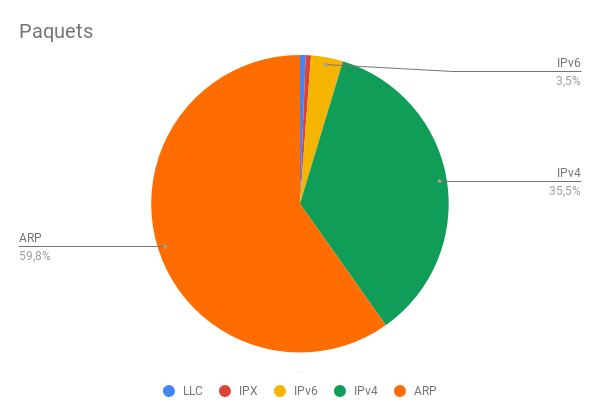
\includegraphics[scale=2]{graphic.png}
\caption{Gràfic de sectors dels protocols de nivell 3}
\label{graph:img}
\end{figure}
\section{Anàlisi nivell de transport}
Abans de començar s'ha de desestimar certs paquets i protocols per a dur
a terme les diferents qüestions. A continuació, s'exposarà 
els filtres que s'utilitzaran per a cada un dels punts.\\
\begin{itemize}
\item Pels paquets que tenen com a destí l'adreça de broadcast de nivell 2,
s'empraràla comanda:
\begin{verbatim}
!eth.dst == ff:ff:ff:ff:ff:ff
\end{verbatim}
\item Pels paquets d'IPv6, s'utilitzarà:
\begin{verbatim}
!ipv6
\end{verbatim}
\item Pels paquets de multicast, s'aplicarà el filtre:
\begin{verbatim}
!(eth.dst[0] & 1)
\end{verbatim}
Que no utilitza la segona clausula donat que el paquets de broadcast
ja han estat eliminats.
\item Pel protocols ARP, DNS i NTP s'emprarà:
\begin{verbatim}
!arp and !dns and !ntp
\end{verbatim}
\end{itemize}
Aplicant totes les condicions obtenim el filtre:
\begin{verbatim}
!(eth.dst[0] & 1) and !arp and !dns and !ntp 
and !ipv6 and !eth.dst == ff:ff:ff:ff:ff:ff
\end{verbatim}
A causa de que l'adreça de broadcast ethernet té el primer valor a 1,
la filtre per a detectar multicast simplifica el filtre fins a tenir:
\begin{verbatim}
!(eth.dst[0] & 1) and !arp and !dns and !ntp 
and !ipv6
\end{verbatim}
\subsection{Connexions TCP no dutes a terme}
S'ha utilitzat el filtre:
\begin{verbatim}
tcp and tcp.flags.reset == 1
\end{verbatim}
Per a veure les connexions que han acabat per resposta del servidor.
Per a les altres connexions, s'ha mirat una per una les converses de TCP,
veient si aquestes havien finalitzat de forma excepcional o si es podia treure
conclusions d'aquests. Per a visualtizar les diferents connexions, s'ha utilitzat
la eina \textit{Statistics > Conversations > TCP}. Amb la informació obtinguda
s'ha elaborat la taula \ref{tcp:failed}.\\\\
\begin{table}[!h]
\centering
\begin{tabular}{|C{2cm}|C{1.5cm}|C{2cm}|C{1cm}|C{3cm}|}
\hline
IP origen  &Port Origen  &IP Destí  &Port Destí  &Motiu Fallida
\\
\hline
172.16.0.112  &34640  &10.35.12.34  &1759  &No hi ha hagut 
resposta per part del destí al SYN
\\
\hline
172.16.0.112  &60158  &10.50.54.87  &9876  &No hi ha hagut
 resposta per part del destí al SYN
\\
\hline
172.16.0.102  &43384  &172.0.16.111  &1759  &No hi ha hagut 
resposta per part del destí al SYN
\\
\hline
84.88.27.7  &80  &172.16.0.113  &42901  &S'ha rebut un paquet amb el flag RST
\\
\hline
172.16.0.109  &33764  &172.16.0.113  &80  &S'ha rebut un paquet amb el flag RST
\\
\hline
172.16.0.105  &44730  &172.16.0.122  &80  &S'ha rebut un paquet amb el flag RST
\\
\hline
172.16.0.106  &42542  &172.16.0.118  &6591  &S'ha rebut un paquet amb el flag RST
\\
\hline
\end{tabular}
\caption{Connexions TCP fallides}
\label{tcp:failed}
\end{table}
S'ha tingut en compte el temps de l'últim SYN enviat i 
el temps de connexió gravat per a decidir s'ha realment 
s'havia perdut la connexió o el paquet de resposta no s'ha
gravat en la sel·lecció de la trama.
\subsection{Connexions TCP completes}
En aquesta subsecció, es diran aquelles connexions TCP que han
sigut completes i com s'han trobat. Per a fer-ho, s'han subdividit
aquelles connexions que són comunicacions HTTP i HTTPS,
i la resta de comunicacions.
\subsubsection{HTTP i HTTPS}
Per a cercar les converses que han tingut alguna connexió TCP, s'ha utilitzat
el filtre:
\begin{verbatim}
tcp.port == 80 or tcp == 443
\end{verbatim}
Una vegada utilitzat, s'ha utilitzat la eina per a veure converses del
Wireshark, amb la opció de només veure les que estiguin dins del filtre,
per a veure quines converses s'han matingut en aquests ports. L'única conversa
en HTTPS és la que té per IP origen i destí els valors 172.16.0.112 i 
213.175.193.206, per a simplificar la taula 
\ref{tcp:http}, s'ha unificat amb una sola taula
en haver-se esmentat ja els valors.
\begin{table}[!h]
\centering
\begin{tabular}{|c|c|}
\hline
IP origen &IP destí\\
\hline
172.16.0.109 &10.69.4.176\\
\hline
172.16.0.109 &91.195.125.127\\
\hline
172.16.0.109 &147.91.204.28\\
\hline
172.16.0.109 &13.219.28.2\\
\hline
172.16.0.109 &94.75.223.121\\
\hline
172.16.0.109 &129.177.13.120\\
\hline
172.16.0.109 &5.135.162.176\\
\hline
172.16.0.109 &178.33.193.139\\
\hline
172.16.0.109 &91.210.88.42\\
\hline
172.16.0.109 &217.31.202.63\\
\hline
172.16.0.112 &209.132.181.16\\
\hline
172.16.0.112 &213.175.193.206\\
\hline
172.16.0.112 &84.88.27.7\\
\hline
\end{tabular}
\caption{Conversacions completes en HTTP i HTTPS}
\label{tcp:http}
\end{table}
\subsubsection{Connexions no HTTP i HTTPS}
Per a dur a buscar aquestes connexions, s'ha utilitzat el filtre:
\begin{verbatim}
!(tcp.port == 80 or tcp.port == 443)
\end{verbatim}
Utilitzant el mateix procediment d'abans, s'ha emprat la eina de Converses del
Wireshark i s'han mirat una per una si les connexions eren completes o no.
Amb aquesta premisa s'ha extret l'anàlisi de la taula \ref{tcp:!htpp}.
Per a calcular l'MTU, s'ha afegit 40 bytes al camp proporcionat pel
protocol TCP sobre el segment més llarg, a causa de la mida de les capçaleres
mínima de les capçaleres TCP i IP (20 bytes cada una).\\
\begin{table}[!h]
\centering
\begin{tabular}{|c|c|c|C{1.3cm}|c|c|c|C{1.3cm}|}
\hline
\multicolumn{4}{|c|}{Origen}  &\multicolumn{4}{c|}{Destí}\\
\hline
IP &Port &MTU &Finestra inicial &IP &Port &MTU &Finestra inicial\\
\hline
172.16.0.102 &48009 &1500 &14600 &172.16.0.105 &9642 &1500 &14480\\
\hline
172.16.0.104 &36664 &1500 &14600 &172.16.0.111 &1759 &1500 &14480\\
\hline
172.16.0.104 &45737 &1500 &14600 &172.16.0.125 &22 &1500 &14480\\
\hline
172.16.0.105 &52193 &1500 &14600 &172.16.0.108 &7856 &1500 &14480\\
\hline
172.16.0.106 &45874 &1500 &14600 &172.16.0.112 &22 &1500 &14480\\
\hline
172.16.0.106 &52180 &1500 &14600 &172.16.0.108 &7856 &1500 &14480\\
\hline
172.16.0.106 &50316 &1500 &14600 &172.16.0.103 &21 &1500 &14480\\
\hline
172.16.0.106 &38368 &1500 &14600 &172.16.0.115 &7658 &1500 &14480\\
\hline
172.16.0.109 &49608 &1500 &14600 &172.16.0.108 &7856 &1500 &14480\\
\hline
172.16.0.112 &42095 &1500 &14600 &172.16.0.102 &21 &1500 &14480\\
\hline
\end{tabular}
\caption{Conversacions completes no pertanyens a HTTP i HTTPS}
\label{tcp:!htpp}
\end{table}

\subsection{Connexions UDP no dutes a terme}
UDP no és un protocol orientat a connexió, pel que dins del protocol
costarà saber si alguna connexió UDP no s'ha dut a terme. Però, el
protocol ICMP avisa quan algun host, port o destí no ha sigut trobat, donant
així una connexió UDP fallida. Utilitzant el filtre:
\begin{verbatim}
upd and icmp
\end{verbatim}
Trobarem els missatges de xarxa produits per aquest tipus de connexió.
Però, donat que hi ha molts missatges de \textit{Time to live}, i, a causa
de que aquest missatge podria ser tractat per una capa superior, s'ha
desestimat tots aquests paquets treient el seu camp amb el filtre:
\begin{verbatim}
!icmp.type == 11
\end{verbatim}
D'aquesta forma, es facilita adquirir les dades amb les quals,
s'ha efectuat la taula \ref{udp:failed}.
%TODO afegir udp:failed
\begin{table}[!h]
\centering
\begin{tabular}{|c|c|c|c|C{3cm}|}
\hline
\multicolumn{2}{|c|}{Origen}  &\multicolumn{2}{|c|}{Destí} 
&\multirow{2}{*}{Motiu}\\
\cline{1-4}
IP  &Port  &IP  &Port &
\\
\hline
172.16.0.111  &55864  &172.16.0.112  &1034  &Port inabastible
\\
\hline
131.206.192.49  &35430  &172.16.0.113  &33504  &Port inabastible
\\
\hline
130.206.192.49  &54863  &172.16.0.113  &33505  &Port inabastible
\\
\hline
130.206.192.49  &50066  &172.16.0.113  &33503  &Port inabastible
\\
\hline
130.206.192.49  &41967  &172.16.0.113  &33507  &Port inabastible
\\
\hline
130.206.192.49  &41722  &172.16.0.113  &33508  &Port inabastible
\\
\hline
130.206.192.49  &58040  &172.16.0.113  &33509  &Port inabastible
\\
\hline
\end{tabular}
\caption{Connexions TCP fallides}
\label{udp:failed}
\end{table}

% Soc un spaghetti per a que sapigues quan comença les conclusions
% YJUUU
% VOLA
% XAN XAN
% Si Sol fa sol fa mi (Nocture de Chopin)
\section{Conclusions}
\section{Annex}
\begin{table}[!h]
\centering
\begin{tabular}{|C{4cm}|}
\hline
Adreces multicast\\
\hline
ff02::1:ff16:f8e9\\
\hline
ff02::1:ff3a:5c61\\
\hline
ff02::1:ff4e:9436\\
\hline
ff02::1:ff52:275\\
\hline
ff02::1:ff5f:1802\\
\hline
ff02::1:ff62:ce40\\
\hline
ff02::1:ff74:9938\\
\hline
ff02::1:ff84:f581\\
\hline
ff02::1:ff90:170b\\
\hline
ff02::1:ff92:210f\\
\hline
ff02::1:ff9e:c17f\\
\hline
ff02::1:ffac:b684\\
\hline
ff02::1:ffb5:ecdb\\
\hline
ff02::1:ffbf:a6df\\
\hline
ff02::1:ffc8:6083\\
\hline
ff02::1:ffca:c1b3\\
\hline
ff02::1:ffdb:187\\
\hline
ff02::1:ffe1:112f\\
\hline
ff02::1:ffeb:4add\\
\hline
\end{tabular}
\caption{Adreces multicast de format ff02::1:ff00:0/104}
\label{mult:104}
\end{table}
\end{document}





































